\chapter{Implementation}
\label{chap:implementation}

This chapter discusses in detail all the implementation aspects of the framework, showing all its characterizing elements.
First, the reasons for choosing Kotlin as the language to implement the framework are explained.
Then, for each module, the logic governing it, the main classes, and usage scenarios will be analyzed.
Finally, the chapter will conclude with a discussion of the configuration DSL and the platform DSL and how they support the user in the system
configuration.

\section{Languages with multiplatform targets}
\label{sec:languages-multiplatform-targets}

Pulverization is born in the context of CPS where device heterogeneity is a real scenario.
For those reasons, we can deal with networks of embedded devices (which have very limited computational resources) up to networks of computers with
high computational power and memory.
Nowadays, architectures that combine these two scenarios are increasingly common, thus having to manage architecturally heterogeneous networks of
devices.

For these reasons, it is necessary to build a framework that can support a wide range of architectures and platforms to maximize the number
of devices on which the framework can run.

In this context, the choice of the language to implement the framework is crucial.
A cross-platform language (or even known as multiplatform language) is a language that allows the same code to be compiled for different platforms.
The trend over the last years is to use the same language to span over several runtime and VMs (e.g. JVM, JavaScript, native platforms, etc.) in order
to reduce the effort of maintaining the codebase and to increase the portability of the application.
The other main advantage of using a multiplatform language is that all the shared concepts and logic can be implemented in a single codebase that
can be reused in all the specific platforms.

In this way, we can use one programming language and manage the targeting of multiple platforms effectively (see~\Cref{fig:mulitplatform-languages}).

\begin{figure}[h]
	\centering
	\begin{tikzpicture}
		\path[mindmap,concept color=blue!20,text=black]
		node[concept] {Core language}[clockwise from=-33]
		child[concept color=green!20] {
				node[concept] {JavaScript} [clockwise from=-60]
				child { node[concept] {Node.js} }
				child { node[concept] {Web Browser} }
			}
		child[concept color=red!20, level distance=150, clockwise from=-40] {
				node[concept] {Native}
				child { node[concept] {Windows} }
				child { node[concept] {Linux} }
				child { node[concept] {macOS} }
			}
		child[concept color=orange!20] { node[concept] {JVM} };
	\end{tikzpicture}
	\caption{Diagram showing the rationale behind the multiplatform languages.}
	\label{fig:mulitplatform-languages}
\end{figure}

The two following sections will examine two of the main relevant language based on the JVM ecosystem that supports multiplatform targets.

\subsection{Scala Language}
\label{sec:scala-language}

The Scala programming language is a general-purpose programming language that is designed to combine object-oriented and functional programming in one
concise, high-level language.

Although Scala was born under the JVM, it has been extended to support other platforms such as JavaScript, and native platforms.

Support for cross-platform is enabled through external plugins and not directly by the Scala compiler itself.
The plugin enables compiler extensions allowing the generation of \emph{intermediate representations} (IRs) containing platform-specific aspects;
with the IR, the compiler makes optimization, linking and other dependencies management.

The~\Cref{lst:scala-cross-platform} shows the minimal configuration required to enable the cross-platform support for the Scala language,
in particular are enabled JVM, JavaScript and native platforms.

\lstinputlisting[
	float=h,
	language=scala,
	caption={Minimal configuration to enable cross-platform support for Scala.},
	label={lst:scala-cross-platform}
]{listings/scala-cross-platform.sbt}

\begin{figure}[h]
	\centering
	\begin{subfigure}{.45\textwidth}
		\centering
		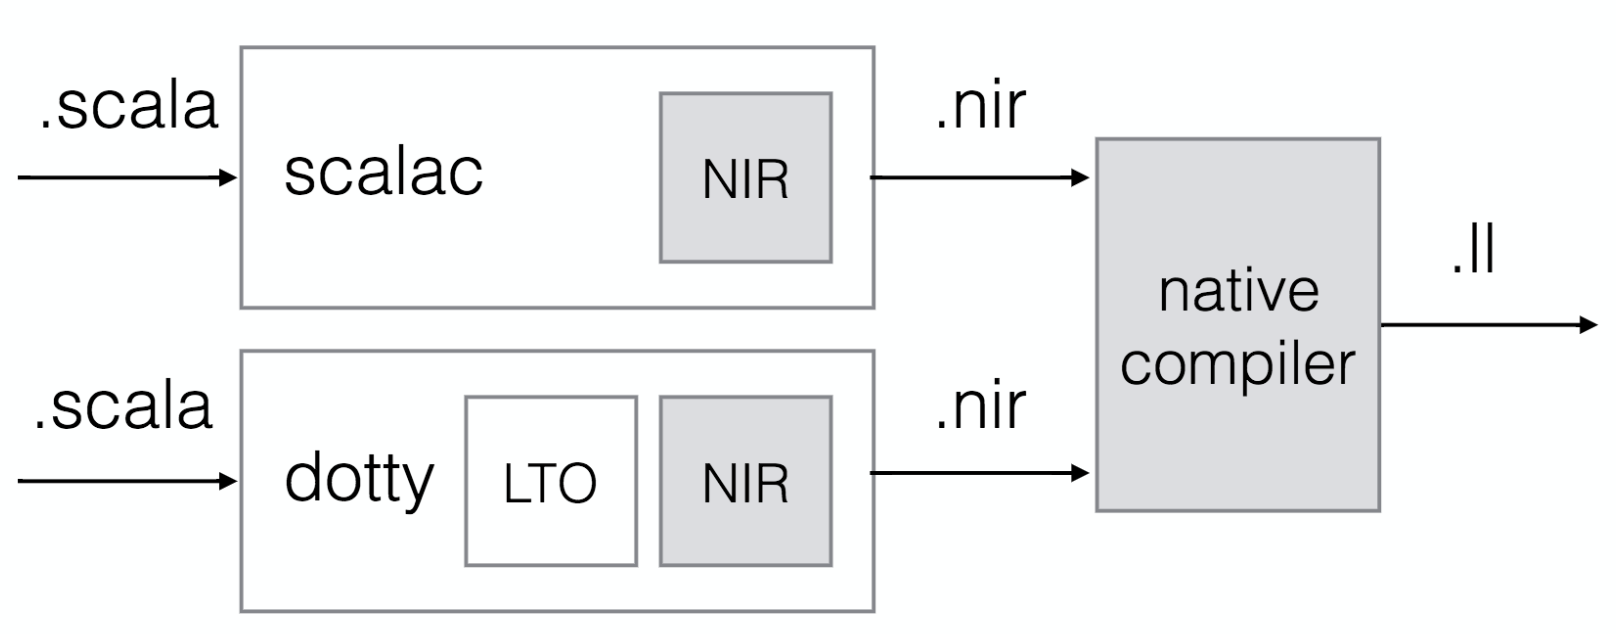
\includegraphics[width=0.95\linewidth]{figures/scala-native-ir.png}
		\caption{Scala native compilation pipeline. Picture taken from~\cite{scala-native-ir}.}
		\label{fig:scala-native-ir}
	\end{subfigure}
	\begin{subfigure}{.45\textwidth}
		\centering
		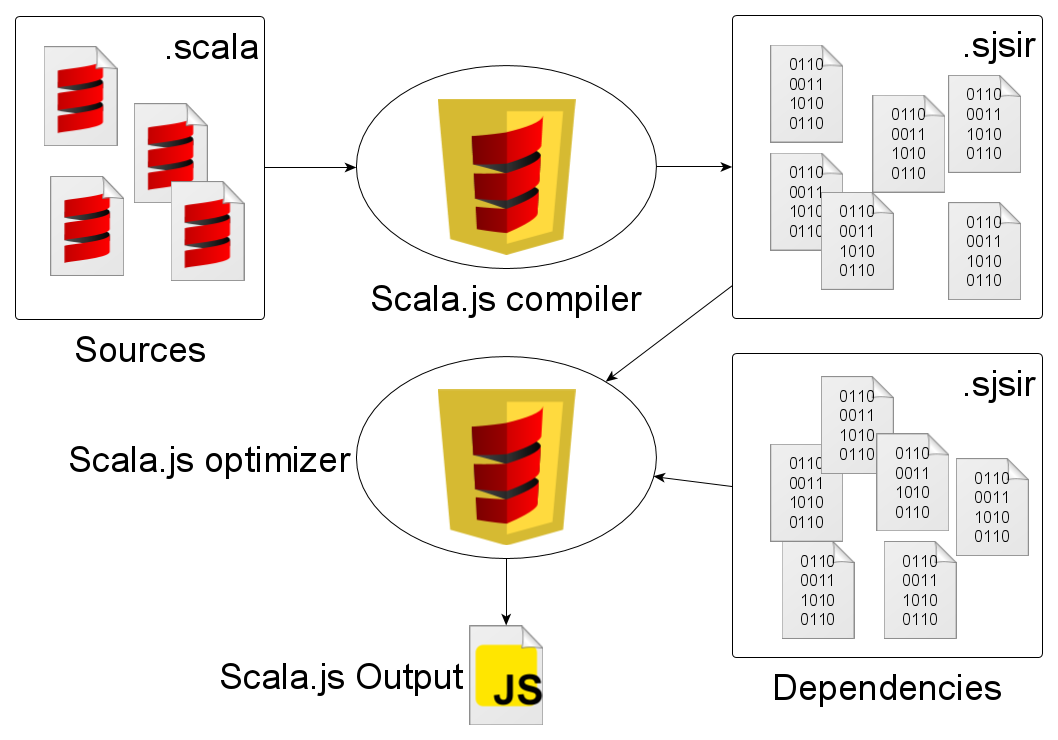
\includegraphics[width=.95\linewidth]{figures/compilation-pipeline.png}
		\caption{Scala.js compilation pipeline. Picture taken from~\cite{scala-js}.}
		\label{fig:scala-js-ir}
	\end{subfigure}
	\caption{Representation of the Scala Native and Scala.js IR generation and compilation pipelines.}
	\label{fig:scala-ir}
\end{figure}

The~\Cref{fig:scala-ir} depicts the two main targets and for each one shows the compilation pipeline in particular, the~\Cref{fig:scala-native-ir}
shows the compilation pipeline for the native target, while the~\Cref{fig:scala-js-ir} shows the compilation pipeline for the JavaScript target.

For what concern the native target, the compilation pipeline is composed of the following steps~\footnote{https://scala-native.org/en/stable/contrib/compiler.html}:
\begin{itemize}
	\item \textbf{Scala code compiled into Native Intermediate Representation:} the \texttt{nscplugin} takes the Scala source code and inspecting the
	      AST, it generates the \texttt{.nir} files.
	\item \textbf{LLVM final compilation:} all the \texttt{.nir} files are compiled into \texttt{.ll} files and passed to the LLVM compiler that
	      produces the native binary file.
\end{itemize}

The pipeline for the JavaScript target is quite more articulated but for the sake of simplicity, are reported only the main phases of the compilation
steps~\cite{Doeraene:256862}:
\begin{itemize}
	\item \textbf{Generation of the Scala.js IR:} the \texttt{scalajs-compiler} takes the Scala source code and generates the \texttt{.sjsir} files.
	\item \textbf{Optimization (linking):} in this phase the \texttt{scalajs-optimizer} takes the \texttt{.sjsir} files and performs optimizations
	      taking also other \texttt{.sjsir} files coming from dependencies.
	\item \textbf{Output file:} the \texttt{scalajs-optimizer} generates the \texttt{.js} file that is the output of the compilation.
\end{itemize}

During the first step, the \texttt{.scala} source files are compiled with scalac, augmented with the Scala.js compiler plugin.
The compiler plugin takes the internal compiler ASTs that have been lowered to contain JVM-style classes, interfaces, methods and instructions, and
turns them into Scala.js IR (\texttt{.sjsir} files).

The \texttt{.sjsir} files are similar to \texttt{.class} files, although they are AST-based (instead of stack-machine-based) and contain features
dedicated to JavaScript interoperability. The \texttt{.sjsir} format and specification are independent of Scala: meaning that the linker is
independent of the language version.

\subsubsection{Scala multiplatform ecosystem}

This section will examine the current ecosystem concerning the multiplatform support for the Scala language to have more awareness about the
usability of this technology.
In particular, will be addressed two main factors: the number of libraries that supports multiplatform targeting and the maturity of each platform.

At first glance, there is a strong sense of fragmentation of projects and communities. Some communities pervasively support all three
platforms (JVM, JS, and native) while others do not, and this is reflected in the amount of multi-targeting compatible libraries.
For example, the \emph{typelevel} ecosystem supports all three platforms for all their main libraries:
\textbf{Cats Effects}~\footnote{\url{https://typelevel.org/cats-effect/}} and \textbf{FS2}~\footnote{\url{https://fs2.io/}}.
From the other side, the \emph{zio}~\footnote{\url{https://zio.dev/}} ecosystem supports only JVM and JavaScript while the native platform is an
experimental stage.
Even if the actual number of libraries is not so high, the Scala ecosystem is quite mature to be used in its multiplatform version.
Moreover, there is a lot of work being done by the Scala community to improve the multiplatform support for the language, so it's very likely that in
the future the number of libraries targeting multiplatform will increase.

To complete the analysis and to have a more complete picture of the Scala multiplatform ecosystem, will be examined the maturity of each platform.
Starting from \emph{Scala.js}, the platform is quite mature and stable: the project was born several years ago and it's used in production by many
companies. Year to year several improvements were made to reach a high level of performance and stability~\cite{marr2016cross}.

Finally, the \emph{Scala Native} platform works quite well but has some limitations that make it not suitable for all production use.
One of the biggest and most important limitations is the lack of support for multithreading~\footnote{\url{https://typelevel.org/blog/2022/09/19/typelevel-native.html}}.
If for some projects this limitation is not a problem, for others it can be a big issue; nevertheless, the \emph{typelevel} community dealt with this
restriction by implementing an event-loop-based concurrency model to support native projects.
Another limitation is represented by the supported architectures: at the time of writing, only a subset of the platforms supported by LLVM
can be targeted, which means that not all the embedded devices can be supported.

\subsection{Kotlin Language}
\label{sec:kotlin-language}

Kotlin is a cross-platform, statically typed, general-purpose high-level programming language.
It's designed to interoperate fully with Java but also compile to JavaScript or native code via LLVM.

Kotlin multiplatform is designed to simplify the development of cross-platform projects by reducing the time spent writing and maintaining the same
code for different platforms.

The Kotlin multiplatform use cases can be synthesized in the following points:
\begin{itemize}
	\item \textbf{Android and iOS applications} sharing the code between mobile platforms enable the building of cross-platform mobile applications
	      sharing the common code between Android and iOS.
	\item \textbf{Full-stack web applications} when building web applications, it's possible to share the code between the client and the server
	      reusing the same logic on both sides.
	\item \textbf{Multiplatform libraries} a multiplatform library with common code and its platform-specific implementations for JVM, JS, and Native platforms can be created. Once published, a multiplatform library can be used in other cross-platform projects as a dependency.
\end{itemize}

\begin{figure}[h]
	\centering
	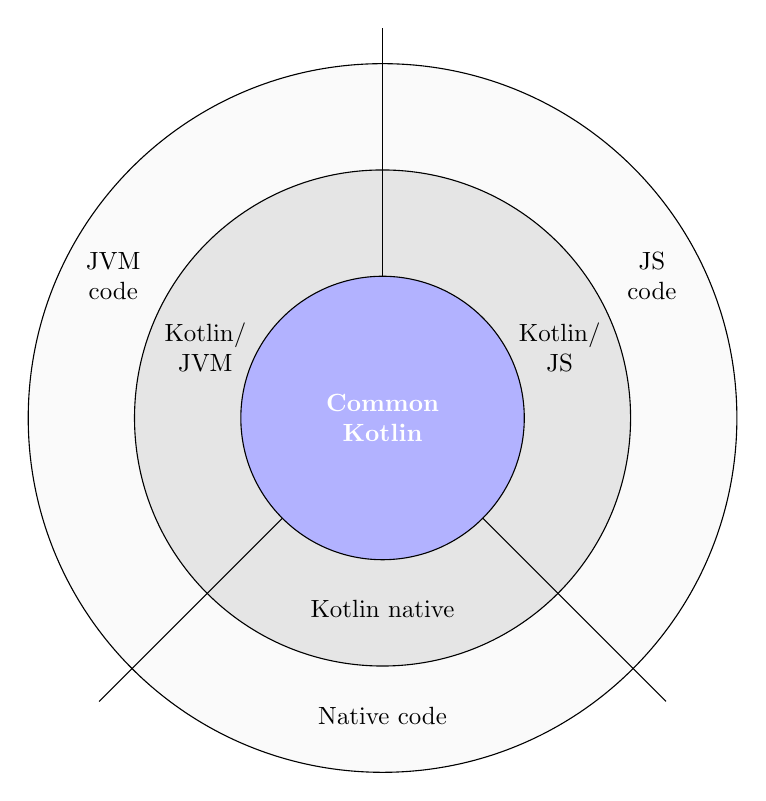
\begin{tikzpicture}[scale=0.9, every node/.style={scale=0.9}]
		\filldraw[fill=black!2] (0,0) circle (5);
		\filldraw[fill=black!10] (0,0) circle (3.5);
		\draw (0,0) -- (0,5.5);
		\draw (0,0) -- (4,-4);
		\draw (0,0) -- (-4,-4);
		\filldraw[fill=blue!30] (0,0) circle (2) node[align=center, color=white, font=\bfseries] {Common\\Kotlin};
		\node[align=center] at (3.8,2) {JS\\code};
		\node[align=center] at (2.5,1) {Kotlin/\\JS};
		\node[align=center] at (-3.8,2) {JVM\\code};
		\node[align=center] at (-2.5,1) {Kotlin/\\JVM};
		\node[align=center] at (0,-2.7) {Kotlin native};
		\node[align=center] at (0,-4.2) {Native code};
	\end{tikzpicture}	\caption{Kotlin multiplatform structure.}
	\label{fig:kotlin-multiplatform-structure}
\end{figure}

The Kotlin multiplatform works using a structure (see~\Cref{fig:kotlin-multiplatform-structure}) where the common code is at the center
and works everywhere on all platforms, and to interoperate with platforms, a specific version of Kotlin is used that includes platform-specific
libraries and tools. Through these platforms, you can access the platform's native code and leverage all native capabilities.

Similarly to Scala, the multiplatform support for Kotlin is enabled via a
Gradle~\footnote{\textbf{Gradle} is a build automation tool for multi-language software development. It's based on \emph{Apache Ant} and
	\emph{Apache Maven} introducing a Groovy and Kotlin DSL. The main supported languages are \emph{Java, Kotlin, Groovy} and \emph{Scala}.} plugin.
As for Scala, the plugin enables a series of tools and compiler extensions to support multiplatform development.

The~\Cref{lst:koltin-multiplatform-setup} shows a basic setup of Kotlin multiplatform using the Gradle plugin.

To share code between all the platforms, Kotlin provides a specific mechanism using a hierarchical structure of modules.
The common code is placed in the \texttt{commonMain} module and it's used to share the common business logic that applies to all the platforms.
Often there is the need to create several native targets that could potentially reuse a lot of the common logic and third-party APIs. Kotlin allows
to create a specific and flexible structure to reuse as much code as possible between the different targets.
The~\Cref{fig:kotlin-multiplatform-hierarchy} shows a possible representation of a Kotlin multiplatform project hierarchical structure.

\lstinputlisting[
	float=ht,
	language=kotlin,
	caption={Minimal Example of Kotlin multiplatform setup using Gradle.},
	label={lst:koltin-multiplatform-setup}
]{listings/kotlin-multiplatform-setup.kts}

\begin{figure}[h]
	\centering
	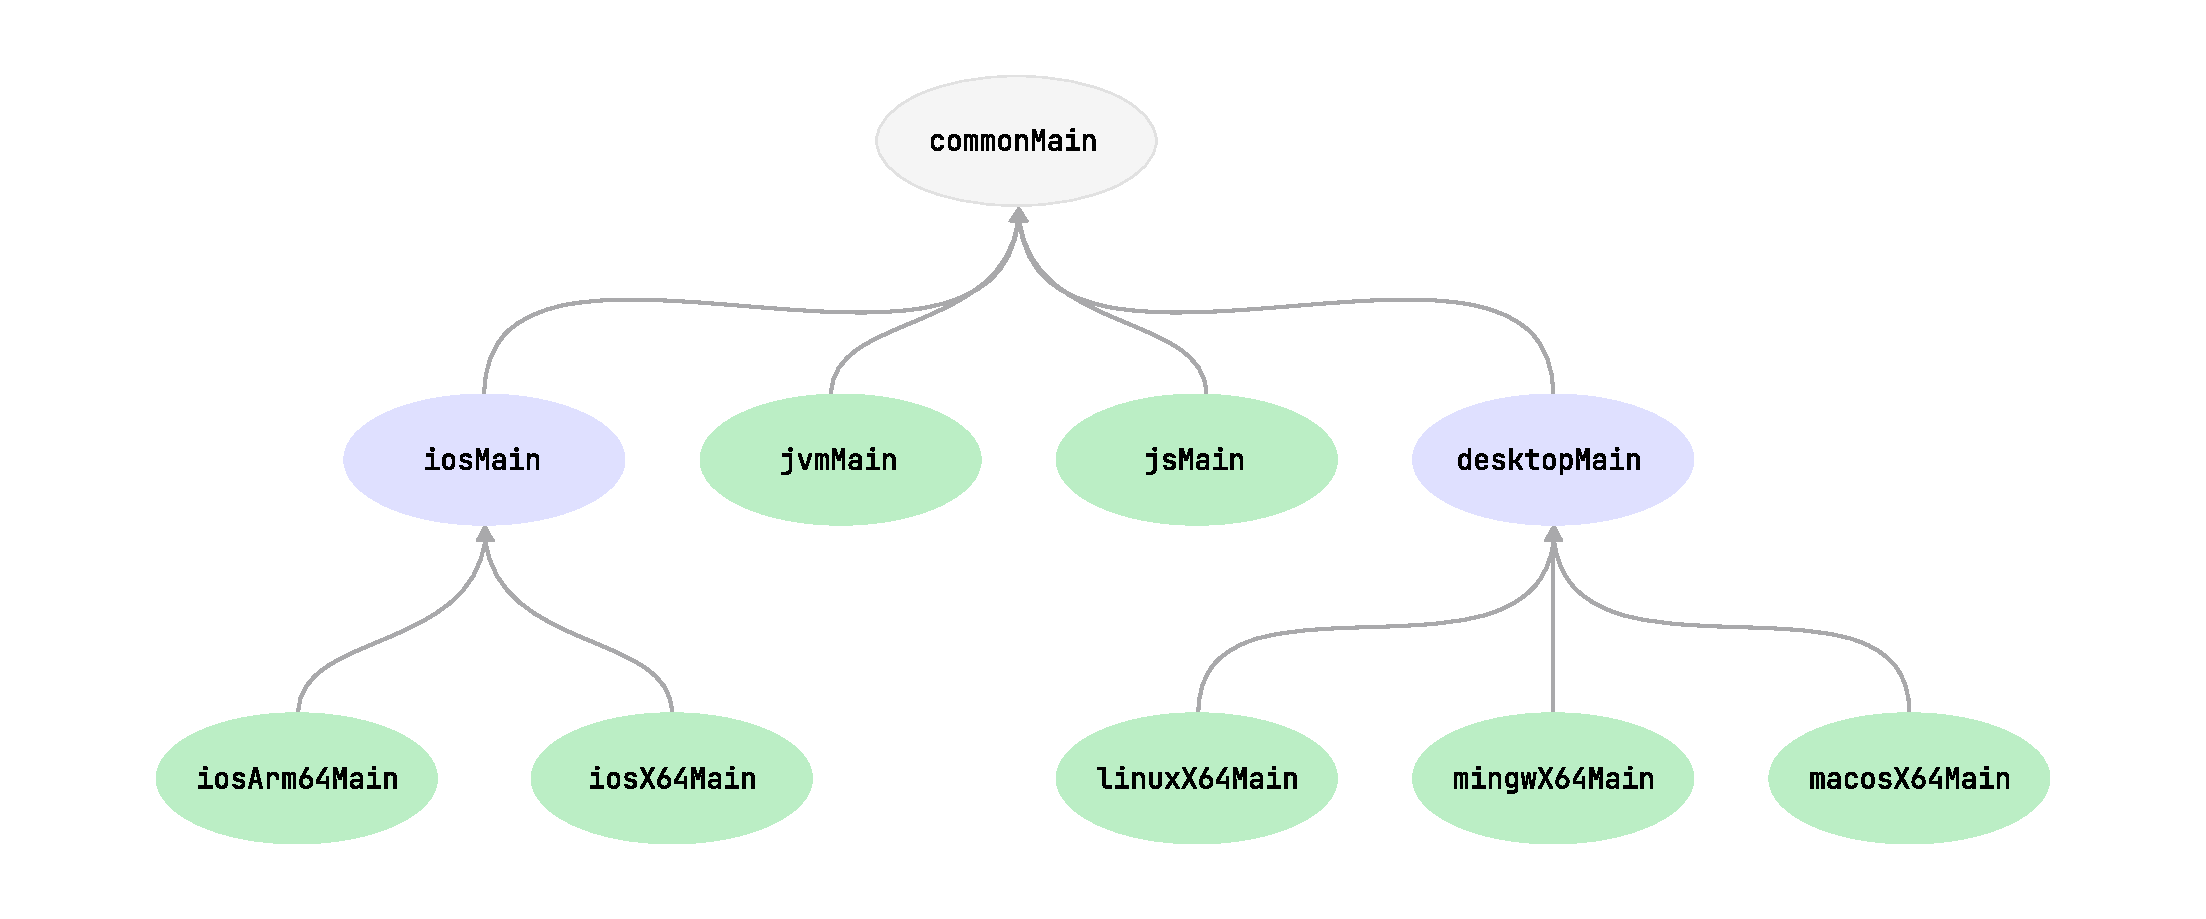
\includegraphics[width=\linewidth]{figures/kotlin-multiplatform-hierarchical-structure.pdf}
	\caption{Kotlin multiplatform hierarchical structure. Picture taken from~\cite{kotlin-package-structure}.}
	\label{fig:kotlin-multiplatform-hierarchy}
\end{figure}

To access the platform-specific APIs from the shared code, Kotlin provides a specific mechanism called \emph{expect/actual}
declarations~\footnote{\url{https://kotlinlang.org/docs/multiplatform-connect-to-apis.html}}.
With this mechanism, a common source set defines an expected declaration, and platform source sets must provide the actual declaration that
corresponds to the expected declaration.

\begin{figure}[h]
	\centering
	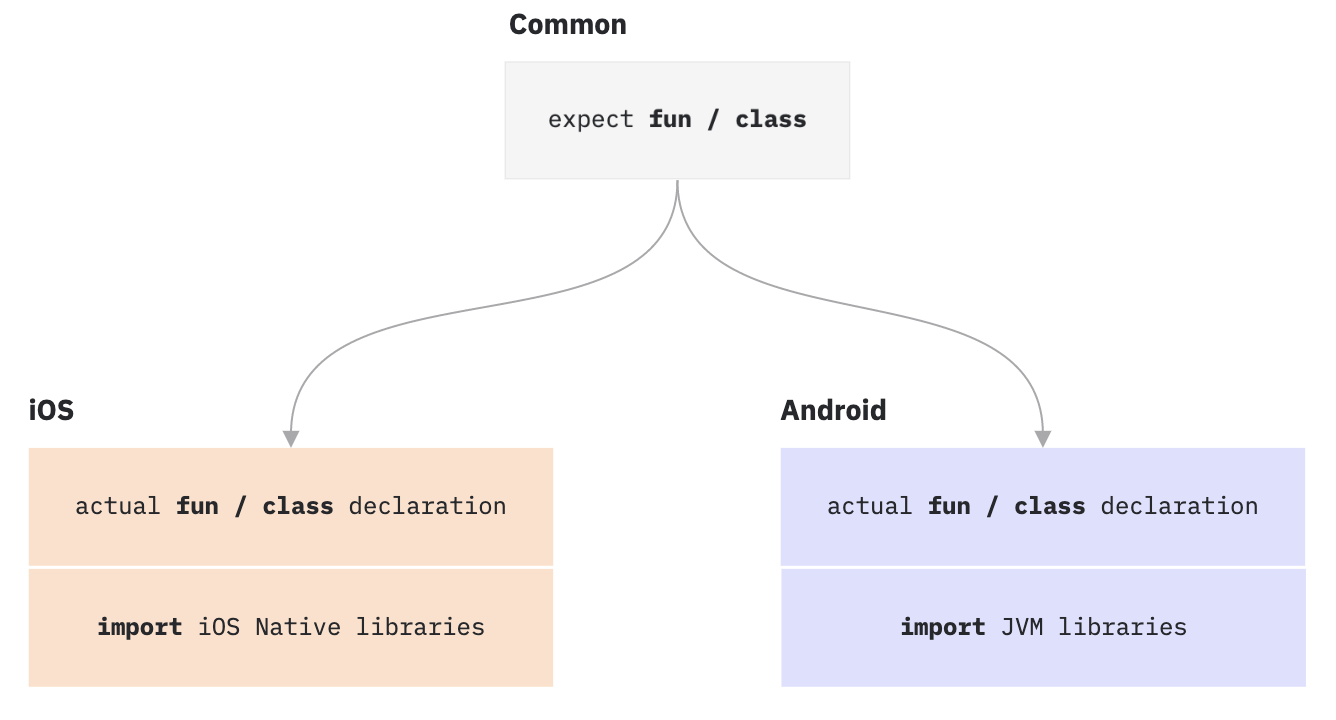
\includegraphics[width=\linewidth]{figures/expect-actual.png}
	\caption{Kotlin multiplatform expect/actual mechanism. Picture taken from~\cite{kotlin-expect-actual}.}
	\label{fig:kotlin-multiplatform-expected-actual}
\end{figure}

The \emph{expect/actual} mechanism is shown in~\Cref{fig:kotlin-multiplatform-expected-actual} where a class in the common source set is marked as
\texttt{expect} and the platform-specific source set provides the actual implementation of the class leveraging platform-specific API.

The compiler ensures that every declaration marked as \texttt{expect} has a corresponding declaration marked as \texttt{actual} in the corresponding
platform modules. In this way, is guaranteed that every platform has an implementation for that class or function.

The following will be a brief introduction to how Kotlin can generate native code and js code from the same code base.

The \emph{Kotlin/JS IR} compiler is responsible for compiling Kotlin code into JavaScript code. The compiler backend rather than generating directly
JavaScript code generates an intermediate representation (IR) of the code which is subsequently compiled into JavaScript code.
This strategy enables aggressive optimizations, improving, for example, the generated code size.

Similarly, the \emph{Kotlin/Native} compiler is responsible for compiling Kotlin code into native code. The compiler is available for all the main
operating systems (macOS, Linux, and Windows) and supports different targets like \textbf{iOS, Windows, macOS, Linux, Raspberry PI,} and
\textbf{WebAssembly}. Unfortunately, there aren't details about how the compiler pipeline works, but it's possible to see that the compiler generates
an IR representation of the code and then compiles it into native code via LLVM.
A relevant feature of \emph{Kotlin/Native} is the interoperability with \emph{C} code. This feature allows using existing C libraries in Kotlin using
the \emph{cinterop} tools by generating Kotlin bindings for the C library. The \emph{cinterop} tool requires a \texttt{.def} file that describes what
\texttt{.a/.so} libraries to include in the build and the corresponding \texttt{.h} files to parse. Finally, the \emph{cinterop} tool generates a
Kotlin library that can be used in the Kotlin code.

When a \emph{Kotlin/Native} library is distributed, a special file with extension \texttt{.klib} is generated. This file contains all the information
and file specifics for each platform. It's a \texttt{.zip} file containing a predefined directory structure: given the \texttt{foo.klib} file, when
unpacked as \texttt{foo/}, contains the following files and directories:
\begin{itemize}
	\item in the folder with the \emph{component name} is contained the serialized Kotlin IR
	\item in the folder \texttt{targets} are placed the platform-specific files, in particular in the folder \texttt{kotlin} there is Kotlin compiled
	      into LLVM bitcode; in the \texttt{native} folder there are the bitcode files of additional native objects
	\item the \texttt{linkdata} folder contains a set of \emph{ProtoBuf}~\footnote{Protocol Buffers (Protobuf) is a free and open-source
		      cross-platform data format used to serialize structured data.} files with serialized linkage metadata
	\item the \texttt{resources} folder contains resources such as images, fonts, and other files
	\item the \texttt{manifest} file in the java property format describing the library.
\end{itemize}

This structure allows having a single \texttt{.klib} file that can be used on different platforms without the need to recompile the library for each
one of them. In a sense, the \texttt{.klib} file is a portable binary format that can be used on different platforms.

\subsubsection{Kotlin multiplatform ecosystem}

As already done for Scala, the ecosystem will be examined for Kotlin to get a better awareness of the usability of this technology.
Again, the number of supported libraries and the maturity of the framework will be considered to evaluate the adoption of this technology.

Differently from the Scala multiplatform ecosystem, the Kotlin one seems to be more coherent and structured: lots of libraries
like \textbf{kotlinx.serialization}, \textbf{kotlinx.coroutines}, and \textbf{ktor} are available for all the target platforms supported by Kotlin.
The other difference is that most of the libraries are developed directly (or with the support of) the Kotlin team, meaning that support and the
development is more aligned and coherent with the language itself.
The identification of the magnitude of libraries targeting Kotlin multiplatform is quite simple since a
site~\footnote{\url{https://libs.kmp.icerock.dev/}} collects all the available Kotlin multiplatform libraries. From this site can be seen that more
than 140 libraries are available for Kotlin multiplatform, spacing from different categories and applications. Of course, not all the available
libraries are collected on this site, but it's a good starting point to get an idea of the ecosystem.

For concern the maturity of the framework, the Kotlin multiplatform is still in beta, nevertheless, its stability and usability make it a
good candidate for a production-ready product. The Kotlin team is working hard to improve the framework and make it more stable and usable.
If in Scala the specific module for each supported platform (JS and native) is developed by an external community, reducing the guarantee of stability
and coherence with the language, in Kotlin the multiplatform module is developed by the JetBrains team itself, increasing the guarantee of stability
of the entire framework.

\subsection{Why Kotlin multiplatform as a choice}

This section will present the reasons that led to the use of Kotlin as a language for the framework implementation instead of Scala.
The decision was based on three main factors: the \emph{support} of the overall multiplatform ecosystem, \emph{libraries availability} with
multiplatform support and the number of \emph{supported platforms} by each language.

As for \emph{support} related to Scala multiplatform, the issue is controversial. On the one hand, there's Scala.js, which has always been
supported and maintained and has reached a very high level of maturity over time. On the other hand, scala native is managed by another community that
has contributed to the project in a seesaw manner over time, where in some cases the project had even been abandoned.
On the other side, Kotlin multiplatform is entirely supported by JetBrains and is constantly evolving and improving. JetBrains has proven over time
to carefully curate its products ensuring very high-quality standards, a symptom that Kotlin multiplatform may also fall into this case.

The \emph{availability} of libraries that support multiplatform is a key aspect to consider: having a large number of supported available libraries
could be strategic to develop complex applications.
In this regard, the Kotlin multiplatform has a clear advantage over Scala multiplatform: the Kotlin ecosystem is much more structured and coherent
than the Scala one. The Kotlin team has developed a large number of libraries that support multiplatform, and the community has also contributed to
the development of many other libraries.

Finally, the \emph{number of supported platforms} is the most important factor to consider: without extensive support of the most common
architectures and platforms, the adoption of the pulverization framework could be limited.
In this regard, Scala native is not clear about which specific targets supports or it will support in the future, but for sure currently, it does not
support all the Apple mobile ecosystem like iOS, watchOS and tvOS. On the other hand, Kotlin native has wide support for the Apple mobile ecosystem
and also for the Linux platform targeting ARM32, ARM64 and x86\_64 architectures as well as for the Windows platform targeting x86 and x86\_64
architectures.

For all the reasons mentioned above, Kotlin multiplatform was chosen as the framework implementation language.

\section{Technologies used in the framework}

This section offers a comprehensive summary of the various technologies employed across the framework's different modules. Specifically, the key
libraries and mechanisms used in the framework will be highlighted, with a focus on those that are shared across all modules. It should be noted that
technologies and dependencies unique to each module will be discussed in their respective sections.

\subsection{Kotlin coroutines}

Asynchronous programming returned to the mainstream in recent years. Created in the `80s, but with the advent of multi-core processors, it has been
superseded by multi-threaded programming, which was the de facto standard for concurrent computations.
Since the 2000s, lots of programming languages have introduced asynchronous programming features from the start while other languages have added
support later.

Multithreading is a traditional method of performing multiple computations in parallel by executing each computation in a separate thread. However,
it has drawbacks such as increased programming complexity and reduced performance for tasks that are IO-bound.
Different flavours of asynchronous programming are an alternative to multithreading. Unlike multithreading, which is based on coarse-grained threads,
asynchronous programming is implemented via fine-grained suspendable computations, which can more effectively interleave with each other.
Different attempts have been made over the years to provide programming languages with facilities to support asynchronous programming:
\emph{callbacks, futures} and \emph{promise} are only some of the most common approaches.
A callback is a function defined by the user, passed to a callback-aware API as a function value, lambda, function pointer, etc., with the purpose of
being called at a later time when a certain condition is met. Although this is a rather simple mechanism, callback-based frameworks are known to
suffer from a complication of code structure disproportionate to the complexity of the logic that code expresses, commonly referred to as ``callback
hell''~\cite{7321196}. Futures and promises are a step above callback-based computations, working as special proxies for not-yet-completed results
of asynchronous computations. The two main operations that can be performed on a promise are: checking for completion and getting the result of the
computation. Promises are a good solution to the callback hell problem, but they are not without their problems: they are not composable, and they
lack a way to express dependencies between asynchronous computations. \emph{async/await} is an approach that brings asynchronous programming as a
first-class language citizen: \emph{async/await} is based around expressing asynchronous computations as two interconnected parts.

The first language to introduce \emph{async/await} was C\#. A lot of programming languages used the C\# approach as an inspiration and follow its
async/await implementation. JavaScript, TypeScript, Dart, Python, Rust — all these languages use async functions containing await operators.

As follow is introduced the concept of the coroutine and how it is implemented in Kotlin, discussing the basic building block for asynchronous
programming.

Even though the concepts of \emph{coroutine} being used for over 50 years, there is no standard definition of what a coroutine is.
One valid definition could be ``function which can suspend and resume its execution, preserving the state between suspensions''
\cite{elizarov2021kotlin}. Coroutines have been classified using the following axes, where implementations may differ:
\textbf{Symmetric/Asymmetric Control Transfer} and \textbf{Stackfull/Stackless Implementation}.

Symmetric coroutines can suspend themselves and resume the execution to an arbitrary coroutine, in this context the control transfer between
coroutines is symmetrical. On the other hand, asymmetric coroutines can only suspend themselves and resume the execution to the coroutine that
suspended them, in this context the control transfer between coroutines is asymmetric. While symmetric coroutines are more expressive than asymmetric
coroutines, they are also more complex to understand, for this reason, most of the implementation of coroutines are
asymmetric~\cite{elizarov2021kotlin}.

A stackful coroutine implementation allows for suspension at any point within nested functions and, when resumed, continues execution from the exact
point of suspension, restoring the original function call stack. Conversely, a stackless implementation can only be suspended within itself,
requiring that nested functions also be coroutines for asynchronous execution to occur. The majority of modern languages use stackless coroutines.
While stackful coroutines are more powerful than stackless ones, stackless coroutines can match most (if not the same) capabilities
via careful handling of nested coroutine calls; moreover, stackful coroutines are noticeably harder to implement efficiently.

One important aspect when implementing coroutines is the \emph{error handling} mechanism.
There are two approaches currently used in asynchronous programming, the first one is based on supervision trees, which was pioneered in Erlang,
and involves arranging asynchronous tasks in parent-child trees for desired error propagation. The second approach, structured
concurrency~\footnote{\url{https://250bpm.com/blog:71/}}, aims to transfer the idea of structured programming to asynchronous programming. It connects tasks to
their origins and ensures that the lifetime of a task cannot exceed the lifetime of its origin, thereby establishing a \emph{launcher-launchee}
relation and describing error and cancellation propagation.

Structured concurrency, in comparison to supervision trees, has a fixed error-handling strategy and is therefore less flexible. However, it is more
concise and aligns well with the typical way asynchronous code is written. This is why structured concurrency has gained significant attention in
recent years, either as structured concurrency libraries or as a built-in language feature~\footnote{\url{https://wiki.openjdk.org/display/loom/Structured+Concurrency}}. Kotlin uses the structured
concurrency approach to manage error handling in coroutines.

Kotlin coroutines are built upon the following goals~\cite{elizarov2021kotlin}:
\begin{itemize}
	\item \textbf{Independence from low-level platforms implementation:} Kotlin being a multi-platform language, building its asynchronous support on
	      existing implementations like futures in JVM would lead to interoperability issues between platforms. Therefore, a unique approach is
	      necessary to ensure seamless asynchronous support across all platforms.
	\item \textbf{Adaptability to existing implementation:} a strong emphasis is placed on interoperability with existing code, particularly with
	      Java code on the JVM platform. To ensure a smooth experience for developers, Kotlin should support seamless integration of established
	      asynchronous APIs, such as promises in JavaScript or non-blocking input/output in JVM.
	\item \textbf{Support for pragmatic asynchronous programming:} the popularity of the async/await approach in asynchronous programming highlights
	      the significance of code readability. Although less expressive than full coroutines, async/await offers adequate coverage for practical use
	      cases and improved performance.
\end{itemize}

\lstinputlisting[
	float=h,
	language=Kotlin,
	label=lst:example-suspending-function,
	caption={Example of a suspending function.},
]{listings/coroutine-example.kt}

Kotlin asynchronous programming is built around the ``suspending function'' concept, similar to the ``async function'' concept in JavaScript.
A suspending function is marked with the \texttt{suspend} modifier and can be called from other suspending functions. However, their call sites
are \emph{not marked} as \texttt{await}, i.e., calls to suspending functions are implicitly awaited.
In this way, the problem of ``forgotten await'', characterizing the \emph{async/await} approaches, is avoided.

The~\Cref{lst:example-suspending-function} shows an example of a suspending function, which is called from another suspending function showing how
in Kotlin suspensive functions are called implicitly.
In the example can be seen that the suspending function is implicitly awaited, and the result is returned to the caller.

As follow, a brief introduction to how Kotlin coroutines are implemented is presented.
Each suspendable function goes through a transformation from normally invoked function to a continuation-passing style (CPS).
For a suspendable function with $p_1, p_2, \dots, p_n$ parameters and result type $T$, a new function is generated with an additional parameter of
type \texttt{Continuation<T>} and the return type change to \texttt{Any?}.
Also, the calling convention changes: the function may either \emph{suspend} or \emph{return}. When the function returns some result, this result is
directly returned from the function (as usual); if the function suspends, it returns the special value \texttt{COROUTINE\_SUSPENDED}.
The compiler takes care of the transformation, so the developer does not need to worry about it. When the user wants to suspend a coroutine's
execution, they access the coroutine's continuation by calling an intrinsic function \texttt{suspendCoroutineUninterceptedOrReturn}. Then, stores the
continuation object to resume it later. Finally, pass the \texttt{COROUTINE\_SUSPENDED} the intrinsic which is then returned from the function.

Kotlin implements suspendable functions as state machines since such implementation does not require runtime support.
While being able to wrap different existing frameworks for asynchronous computations, Kotlin coroutines also allow writing asynchronous code in
different styles: \emph{async/await} style, using \emph{Channels} or \emph{Generator.}

Coroutines were widely used in the framework to implement asynchronous behaviors idiomatically in Kotlin. In addition, since in the framework, the
exchange of messages between components can occur asynchronously, this was captured through a coroutine-based construct called
Flow~\footnote{\url{https://kotlinlang.org/docs/flow.html}}.

Kotlin Flow is a new addition to the Kotlin coroutines library, and it provides a way to perform asynchronous, sequential computations that emit
values and can be transformed into streams. A Flow is a sequence of values that are emitted asynchronously and can be processed in a non-blocking
manner. Unlike traditional streams, Flows are also cancellable, meaning that they can be stopped at any point in their execution. Flows are designed
to be highly composable, allowing the building of complex, multi-step computations by combining and transforming smaller Flows. They are also
designed to work well with coroutines, making them an excellent choice for asynchronous and reactive programming in Kotlin.

For those reasons, \emph{coroutine} and \emph{Flow} are the main tools used in the framework providing a simple and efficient way to implement
asynchronous behaviors.

\subsection{Dependency Injection: Koin}

Dependency Injection is a software design pattern that allows for the separation of concerns in a software application. It enables the creation of
loosely-coupled code, which is more flexible and easier to maintain. Dependency Injection is achieved through the injection of dependencies, or
required objects, into the objects that need them. This can be done either manually or through the use of a Dependency Injection framework.

One such framework is the \emph{Koin} library, which is a popular, lightweight, and pragmatic Dependency Injection solution for Android and Kotlin.
The library offers a simple and efficient API, with no reflection or code generation required, making it a fast and efficient choice.

Koin uses a modular approach to Dependency Injection, allowing the definition of dependencies in modules, assembling and managing
them easily. This makes it easy to maintain and update dependencies as needed. In addition, Koin offers a range of features, including scope
management, property injection, and support for multi-threading, making it a comprehensive solution for Dependency Injection in Android and Kotlin
projects.

The~\Cref{lst:example-koin} shows how to use Koin to inject a dependency into a class.

\lstinputlisting[
	float=h,
	language=Kotlin,
	label=lst:example-koin,
	caption={Example of Koin usage.},
]{listings/koin-example.kt}

In this example, a data class \texttt{MySimpleClass} is defined, and a module \texttt{myModule} is also defined to provide an instance of the class
as a singleton. The \texttt{startKoin} function is then used to start Koin and use the defined module. Finally, the dependency is injected into
\texttt{MyClass} using the by \texttt{inject()} property delegate. The main function creates an instance of MyClass and prints the message from the
injected \texttt{MySimpleClass.}

The use of Koin in the framework allows for the easy injection of dependencies into the different components of the framework, making it easy to
maintain and update the framework as needed. Moreover, the use of Koin allows for the easy creation of new components, without an excessive amount of
boilerplate code.

% - New section ---------------------------------------------------------------

\section{Core module}
\label{sec:core-module-impl}

The \texttt{core} module models the core concepts of the framework. The~\Cref{fig:core-module-impl} shows the package structure of the module, which
is divided into two main packages: \texttt{core} and \texttt{dsl}.

\begin{figure}[h]
	\centering
	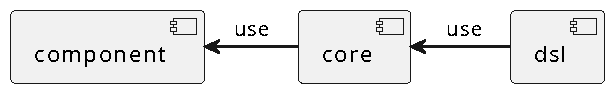
\includegraphics[width=0.7\textwidth]{figures/core-package-diagram.pdf}
	\caption{Core module implementation}
	\label{fig:core-module-impl}
\end{figure}

The \texttt{core} package contains all the interfaces that model the pulverization components.
In particular, in~\Cref{tab:core-interfaces} are listed the fundamental interface defined in the \texttt{core} package.

\begin{table}[h]
	\begin{tabularx}{\textwidth}{l X}
		\toprule
		Interface                   & Description                                                                            \\ \midrule
		\texttt{Behaviour}          & The interface that models the behaviour of a component                                 \\
		\texttt{SensorsContainer}   & The interface that models all the sensors belonging to a device                        \\
		\texttt{ActuatorsContainer} & The interface that models all the actuators belonging to a device                      \\
		\texttt{State}              & The interface that represents the state of a device                                    \\
		\texttt{Communication}      & The interface that models the capability of a device to communicate with other devices \\ \bottomrule
	\end{tabularx}
	\caption{Core interfaces}
	\label{tab:core-interfaces}
\end{table}

All the interfaces illustrated in~\Cref{tab:core-interfaces} are based on another concept expressed by the \texttt{Initializable} interface.
The \texttt{Initializable} interface is used to model the initialization of a component. Every component, before being used, should allocate resources
or perform some operations before becoming operative, as well as release those resources when the component should be destroyed.
The \texttt{Initializable} interface is used to model this concept and is implemented by defining two methods: \texttt{initialize} and
\texttt{finalize}. The former must be invoked before the use of the component, while the latter must be invoked when the component is no longer
needed, during the finalization step of the system.

Analyzing the common aspects of the components defined in~\Cref{tab:core-interfaces}, it is possible to identify another common concept that can
be isolated in a single common interface: the context in which the component is executed. In this specific scenario, the \texttt{Context} interface
holds information about the specific device that components belong to, representing this information with the field \texttt{deviceID}.

All those two concepts are implemented in a third interface that models the concept of ``generic pulverization component'' called
\texttt{PulverizedComponent}, which is the base interface for all the components defined in~\Cref{tab:core-interfaces}.
This interface implements also an external interface named \texttt{KoinComponent}; this interface enables field injection for all the class that
implements it. This feature is used to dynamically inject the \texttt{Context} inside of each component.

\begin{figure}[h]
	\centering
	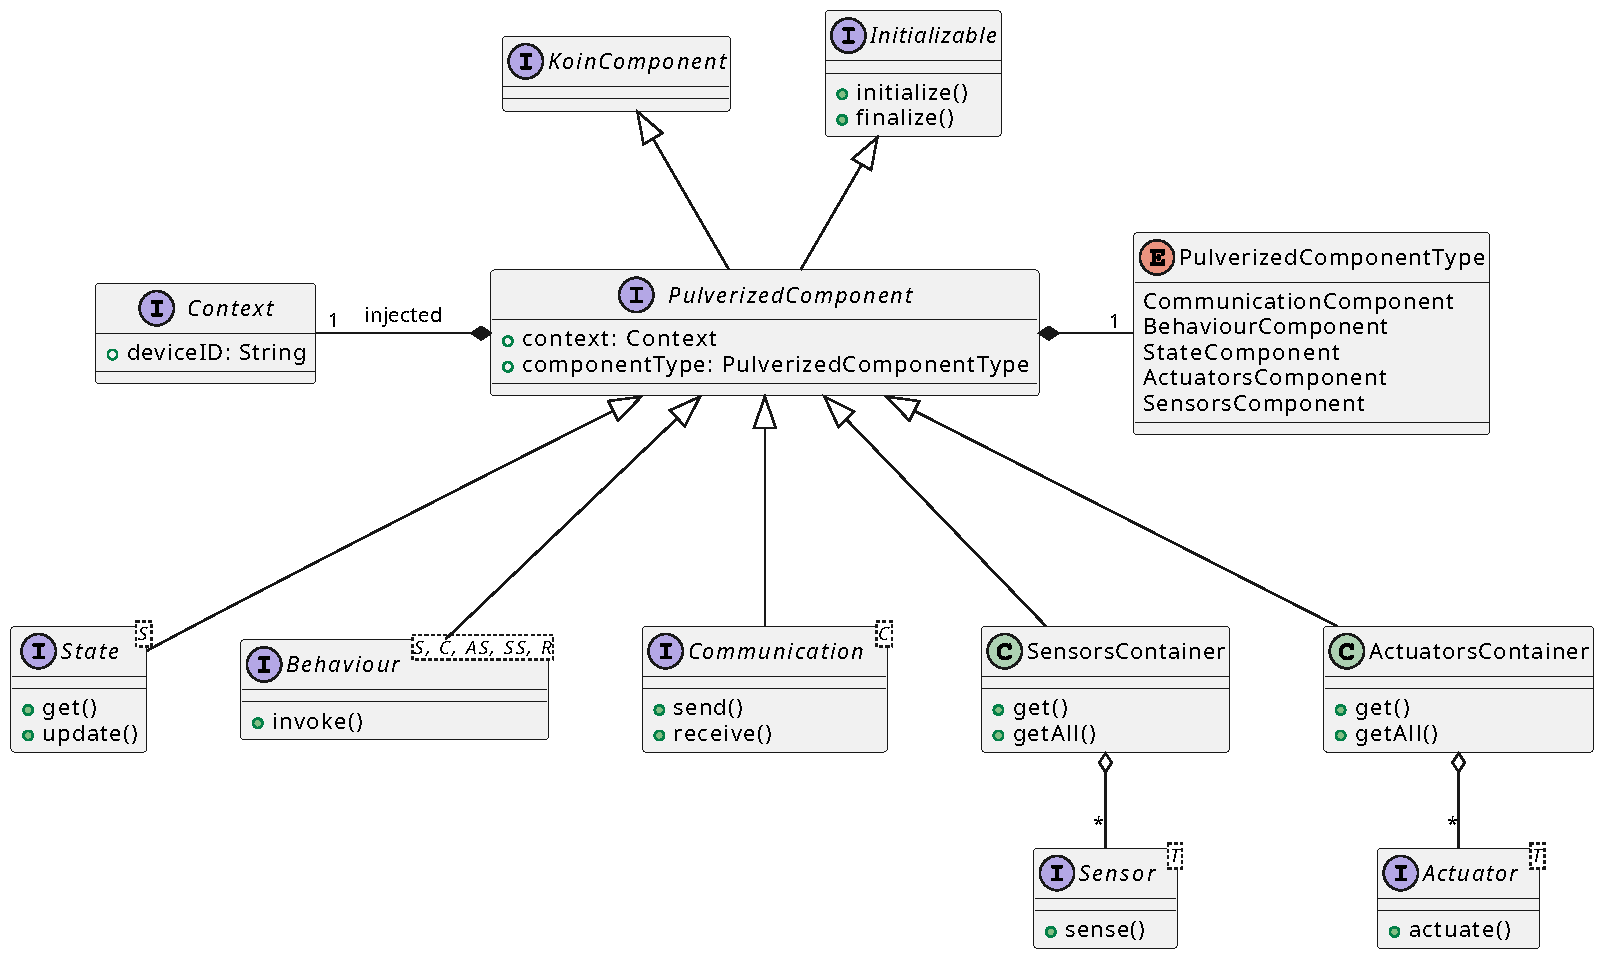
\includegraphics[width=\textwidth]{figures/core-impl-interfaces.pdf}
	\caption{Class diagram showing the relation between the core interfaces of the framework.}
	\label{fig:core-interfaces-class-diagram}
\end{figure}

The~\Cref{fig:core-interfaces-class-diagram} shows the class diagram that models the relationship between the core interfaces of the framework
illustrated previously.

\subsubsection{Sensors and Actuators}

The modeling of the concepts of ``sensors'' and ``actuators'' within the framework and the implementation choices made to model these concepts in the
framework are discussed in more detail below.

All the considerations and choices made to model the concept of \emph{sensor} hold also for the concept of \emph{actuator}, so for the sake of
brevity, only the discussion about the \emph{sensor} concept is reported.

The formulation presented in the original paper~\cite{fi12110203} defines the sensors module as \textit{``a set $\sigma$ of logical sensors''};
starting from this assertion the \textbf{sensor} component is broken down into two separate concepts: the \emph{sensor} which models the physical
sensor from which the data is collected, and the \emph{sensors container} which represents the collector of the sensors belonging to a specific
device.

The \texttt{Sensor} interface, represented in~\Cref{lst:sensor-interface}, models a single sensor defining the method \texttt{sense} which is use to
perform the operation of \emph{sensing the environment.}

\lstinputlisting[
	float=h,
	language=Kotlin,
	caption={Sensor interface defined in the framework.},
	label={lst:sensor-interface}
]{listings/Sensor.kt}

The interface is generic in a type variable \texttt{T} that represents the type of the data collected by the sensor and implements the
\texttt{Initializable} interface to model the ability of initialization of the sensor.

\lstinputlisting[
	language=Kotlin,
	caption={SensorContainer implementation defined in the framework.},
	label={lst:sensor-container-impl}
]{listings/SensorContainer.kt}

More complex and with relevant design choices is the \texttt{SensorContainer} class. The sensors' container is modeled via an abstract class
which implement the \texttt{PulverizationComponent} interface making the container itself initializable.
The storing of the sensors is done via a \texttt{Set} of \texttt{Sensor} objects; since the \texttt{Sensor} interface is generic, it is not possible
to determine which type of sensor will be used, for this reason, the Kotlin type projection over the type variable \texttt{T} of the \texttt{Sensor}
is used. In this way, the \texttt{SensorContainer} can store sensors of different types, and it will be the responsibility of the container to provide
methods that allow retrieving the sensors of a specific type in a type-safe way.
In this regard, the \texttt{SensorContainer} provides three-way of retrieving the sensors: \texttt{get<T>()}, \texttt{getAll<T>()} and
\texttt{get<T>(run)}.
The first method returns a single sensor of type \texttt{T} if it is present in the container, otherwise, it returns \texttt{null}.
This method should be used with care considering that if more sensors with type \texttt{T} are present in the container, only one of them will be
returned with no guarantee on which one will be returned. This method is useful when in the container there is only one sensor of the specified
type.
The second method returns a \texttt{Set} of sensors of type \texttt{T} if at least one sensor of that type is present in the container, otherwise,
an empty \texttt{Set} is returned.
The third method finds the sensor of type \texttt{T} and invokes the \texttt{run} function over the retrieved sensor if it is not \texttt{null},
otherwise, it does nothing.

One of the challenges faced in implementing these methods stemmed from the presence of type erasure.
The type erasure is a feature of the Java virtual machine that removes the type information from the compiled bytecode, making it impossible to
retrieve the type of a generic type variable at runtime. To overcome this limitation, the Kotlin mechanism of \emph{reified type parameters} is used.
This mechanism leverages another mechanism of the Kotlin language called \emph{inline functions} that allows inlining the body of a function
inside the caller function. In this way, a sort of ``local monomorphization'' is performed, allowing the retrieval of the type of the generic type
cleanly, without the need of using reflection via \texttt{KClass<T>}.

Above was discussed the problem of retrieving a sensor in a type-safe way, this problem is solved by inspecting all the objects stored in the
container and returning only those that are an instance of the type \texttt{T}.
The complete implementation of the \texttt{SensorContainer} class is reported in~\Cref{lst:sensor-container-impl}.

As stated above, all the considerations and choices made for the \texttt{Sensor} and \texttt{SensorContainer} are valid also for the \texttt{Actuator}
and \texttt{ActuatorContainer} classes.

\subsubsection{Communication}

The other relevant component in the \emph{core} module is the \textbf{communication} component, which is responsible for the communication between
the devices.
The communication component is described as \textit{``A communication component $\chi$ handling interaction with neighbours, holding information on
	the identity of neighbors and how to reach them, managing input channels used to receive external messages into the device’s state, and output
	channels for emitting messages to all its neighbours''}.
From this description emerges the bidirectional nature of communication where sending and receiving channels are neatly separated.
Another aspect that emerges from the description is the need to hold a reference to the neighbors of the device and their identity.

\lstinputlisting[
	float=ht,
	language=Kotlin,
	caption={Communication interface defined in the framework.},
	label={lst:communication-interface}
]{listings/Communication.kt}

In light of the considerations made above, it was decided to demand the user the responsibility of holding the references to the neighbors and
their identity, and to provide a simple interface to send and receive messages. The rationale behind this choice is that is quite difficult to
provide a generic representation of the network topology and determine how it can change over time, and for this reason, it is better to leave the
responsibility of managing the neighbors to the specific implementation of the communication component.

The \texttt{Communication} interface, presented in~\Cref{lst:communication-interface}, models the communication component and defines
two methods: \texttt{send} and \texttt{receive}.

The interface is generic in a type variable \texttt{P} that represents the type of messages that can be sent and received by the component.
Moreover, the type variable is bounded to the \texttt{Any} type: this captures the fact that the message could not be nullable.
While at first analysis it might seem redundant to specify this type bound, it turns out to be fundamental since in the type hierarchy in Kotlin, the
topmost type is \texttt{Any?} which represents any nullable data type, enabling the possibility of sending and receiving \texttt{null} messages,
a scenario that is not desirable.

While the \texttt{send} method is straightforward, the \texttt{receive} method returns a specific type: \texttt{Flow<P>}.
This type represents an asynchronous stream of values that in this case represents the messages received by all the neighbours.

\subsubsection{Behaviour}

The \textbf{behaviour} component is the heart of the device, it is responsible for the execution of the device's logic.
The behaviour component is described as \textit{``A computation function $\beta$
	modeling the device behavior, which maps the state of the device to a new state, a prescriptive set of actuations to be performed,
	and coordination messages to be emitted''}.

\lstinputlisting[
	float=h,
	language=Kotlin,
	caption={Behaviour interface defined by the framework.},
	label={lst:behaviour-interface}
]{listings/Behaviour.kt}

The \texttt{Behaviour} interface, represented in~\Cref{lst:behaviour-interface}, models the behaviour component and defines a single method:
\texttt{invoke}. Moreover, in the listing are also presented the data classes used to represent the output of the behaviour function.

How the behaviour function should be obtained can be easily inferred from the description above: it should take as input the current state of
the device, the sensed values and the received messages, and it should return the new state of the device, the actuations to be performed and the
messages to be sent. For this reason, the interface is generic in five type variables: \texttt{S} for the state, \texttt{E} for the communication,
\texttt{W} for the sensed values, \texttt{A} for the actuations and \texttt{O} for the outcome of the function.
The output produced by the behaviour function is represented by the \texttt{BehaviourOutput} data class, which is defined
in~\Cref{lst:behaviour-interface}. This class holds information about the new state, the new communication, the actuations to be performed, and the
function's outcome.

The peculiarity of the \texttt{Behaviour} class is that the method \texttt{invoke} is marked as \texttt{operator} which allows the invocation of the
function using the \texttt{()} operator over the class instance.

\subsubsection{State}

Finally, the \textbf{state} component is responsible for the representation of the state of the device.
The state component is described as \textit{``A state $\kappa$, representing the device's local knowledge''}.

\lstinputlisting[
	float=h,
	language=Kotlin,
	caption={State interface defined by the framework.},
	label={lst:state-interface}
]{listings/State.kt}

The framework should abstract the representation of the state of the device, and for this reason, the \texttt{State} interface, represented in
\Cref{lst:state-interface}, models the state component and defines two methods: \texttt{get} and \texttt{update}.
The former is used to retrieve the current value of the state, while the latter is used to update the state with a new value.
Is the responsibility of the user to implement the concrete representation of the state, and for this reason, the interface is generic in a type
variable \texttt{S} that represents the type of the state. Is also the responsibility of the user to persist the state somehow, the reason why the
interface does not provide any details about persistence.

\paragraph*{}

The other relevant construct of this module is the configuration DSL, which will be discussed more in detail in the~\Cref{sec:configuration-dsl-impl}.

% - New section ---------------------------------------------------------------

\section{Platform module}
\label{sec:platform-module-impl}

This module represents the most important part of the framework since it is the one that provides the implementation of the platform.
It is organized in a \emph{communication} package that contains the main abstraction for intra-components communication, a \emph{componentsref}
package which contains all the interfaces needed to uniform the representation of a component reference, a \emph{context} package that contains the
logics for the context creation and, finally, a \emph{dsl} package that contains the DSL used to configure the pulverization platform.
The~\Cref{fig:platform-module} shows the package diagram of the \texttt{platform} module.

\begin{figure}[h]
	\centering
	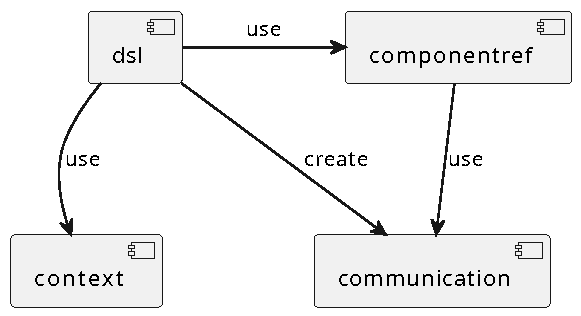
\includegraphics[width=0.7\textwidth]{figures/platform-impl-package.pdf}
	\caption{Package diagram of the \texttt{platform} module showing the relationship between the packages.}
	\label{fig:platform-module}
\end{figure}

\subsubsection{Communication package}

In this package are given the main abstractions for intra-components communication. In particular, the main relevant interface is
\texttt{Communicator}: it is the interface that represents the communication between two components of a logical device.
This interface is developed keeping in mind the fact that the concrete implementation could be based on any kind of communication medium,
and for this reason, specific protocol aspects are abstracted over. This specific abstraction is captured by the \texttt{RemotePlace} data class
that represents the remote place that the receiver's component is deployed on.
This class is composed of two fields named \texttt{who} and \texttt{where:} the former identifies the receiver's component answering the question of
``who is the other component'', while the latter represents where the component is located, answering the question of ``where can I reach the other
components''.
In this way, each communicator will specify how to represent that two fields using protocol-specific aspects: for example, a communicator based on
TCP socket could represent the \texttt{who} field as the IP address of the receiver's component, while the \texttt{where} field could be the port.
In conjunction with the \texttt{RemotePlace} class, the \texttt{RemotePlaceProvider} interface is used to provide the specific remote place based
on the specific protocol and context. The interface provides a method \texttt{get} that takes as input a \texttt{PulverizedComponentType} and
return a \texttt{RemotePlace} if any. The implementation of this interface is demanded by the specific communicator implementation.

The \texttt{Communicator} interface, reported in~\Cref{lst:communicator-interface}, has a \texttt{setup} method that accept as arguments respectively
the \texttt{Binding} and a \texttt{RemotePlace};
those two arguments are used to set up the communication between the two components (defined by the \texttt{Binding}) and how to establish
the connection (using the \texttt{RemotePlace}). The \texttt{finalize} method is used to close the connection between the two components and release
resources if any.

\lstinputlisting[
	float=h,
	language=Kotlin,
	caption={Communicator interface},
	label={lst:communicator-interface}
]{listings/Communicator.kt}

The framework, by default, provides an implementation of the \texttt{Communicator} interface called \texttt{LocalCommunicator} that is used to
implement the communication between two components that coexist in the same deployment unit. This implementation is based on the use of
\texttt{Flow} which represents an asynchronous flow, in particular, two \texttt{Flow} are used to implement the communication: one for receiving
messages (\texttt{inbox} flow) and one for sending messages (\texttt{outbox} flow).
The \texttt{outbox} flow is used by the \texttt{fireMessage} method to send messages to the other component, while the \texttt{inbox} flow is used
by the \texttt{receiveMessage} method to receive messages from the other component.
This specific implementation is used by the platform to enable communication between components in memory in the same deployment unit.

An important aspect to consider is the fact that the \texttt{Flow}s used by the \texttt{LocalCommunicator} should be shared across all the local instances otherwise each instance will have its own \texttt{Flow} and the communication will not occur. To overcome this issue the
\texttt{LocalCommunicator} uses another class called \texttt{CommManager} which is responsible for managing the \texttt{Flow}s.
The \texttt{CommManager} is a singleton that is used to create the \texttt{Flow}s and to share them across all the local instances.
The \texttt{CommManager} relies on the \texttt{lazy} property of Kotlin to create the \texttt{Flow}s only when they are needed and give the same flow
instance on subsequent calls. The \texttt{lazy} property can guarantee a different level of thread safety, in particular, the \texttt{lazy} property
accepts a parameter of type \texttt{LazyThreadSafetyMode} which specifies the behaviour of the lazy property. In this case, is specified
\texttt{LazyThreadSafetyMode.PUBLICATION} which means that the \texttt{Flow} will be created only once and the same instance will be returned on
subsequent calls, obtaining the desired behaviour.

\subsubsection{Componentsref package}

In this package are modeled the interfaces that are used to represent a component reference.
In the framework, the concept of ``component reference'' is introduced to abstract over specific aspects like the protocol used to communicate with
the component and the way how a component can be reached.

\lstinputlisting[
	float=ht,
	language=Kotlin,
	caption={ComponentRefImpl class},
	label={lst:componentref-impl}
]{listings/ComponentRefImpl.kt}

The \texttt{ComponentRef} interface is the main interface that represents a component reference; is generic in a type parameter \texttt{S} that
represents the type of message that the component can send and receive. Even in this case, the type parameter is bounded to \texttt{Any} to prevent
the use of nullable types. The interface provides three main methods: \texttt{sendToComponent, receiveFromComponent} and
\texttt{receiveLastFromComponent}.

This interface is entirely managed by the platform which is responsible for creating the component reference and for providing the right
implementation based on the context in which the component is deployed. For this reason, the end user should not care about the implementation
of this interface and should not extend or implement it. As a design choice, all the implementations of this interface are marked as
\texttt{internal} so that they are not visible outside the platform module.

The \texttt{ComponentRef} interface can be used in two main scenarios: the first one is when the component to which we refer exists in the same
deployment unit or remotely, and the second one is when the component to which we refer not exists at all (e.g when a device does not have one of the
five components).

For the first scenario, the \texttt{ComponentRefImpl} provides an implementation of the \texttt{ComponentRef} interface, while the second scenario is
handled by the \texttt{NoOpComponentRef} that is an implementation of the \texttt{ComponentRef} interface that does nothing
(see~\Cref{lst:componentref-impl}).

The \texttt{ComponentRefImpl} defines a three-argument constructor that accepts respectively a \emph{serializer}, a \emph{binding} and a
\emph{communicator}. The \emph{serializer} is used to serialize and deserialize the messages that the component can send and receive, while the
\emph{binding} is used to identify the component to which we refer (and consequently the source component) and the \emph{communicator} is used to
establish the communication between the two components.
The implementation of this class is quite straightforward, in particular, the \texttt{sendToComponent} method uses the \texttt{fireMessage} method of
the \emph{communicator} to send the message to the other component, while the \texttt{receiveFromComponent} and \texttt{receiveLastFromComponent}
methods use the \texttt{receiveMessage} method of the \emph{communicator} to receive messages from the other component.
The serializer is used to serialize and deserialize the messages that the component can send and receive, while the binding is used to
setup the communicator.
A notable aspect is how the serializer is managed: the serialization is managed via a Kotlin compiler plugin which enriches any class annotated with
\texttt{@Serializable} with the corresponding serializer; in this way on any serializable class can be used the method \texttt{serializer<C>()} to
retrieve the serializer of the class, but this method is inline so can not be used in the constructor of the \texttt{ComponentRefImpl} class because of
type erasure.
To overcome this issue, inside the \emph{companion object} of the class is defined the operator \texttt{invoke} as an inlined function that
accepts only the \emph{binding} and \emph{communicator} as parameters, while the \emph{serializer} is obtained via the reified type, using the
aforementioned \texttt{serializer} method. Since the operator \texttt{invoke} enable the use of the \texttt{()} operator, the class constructor is
emulated reducing the boilerplate needed to create the class.

\lstinputlisting[
	float=h,
	language=Kotlin,
	caption={NoOpComponentRef class},
	label={lst:noopcomponentref-impl}
]{listings/NoOpComponentRef.kt}

The implementation of the \texttt{NoOpComponentRef}, shown on the~\Cref{lst:noopcomponentref-impl}, provides a no-ops implementation of the
\texttt{ComponentRef} interface. The implementation provides that the send operation does nothing, while the receive operations always return
\texttt{null} for the \texttt{receiveLastFromComponent} and an empty flow for \texttt{receiveFromComponent} method.

\subsubsection{Context package}

The context package defines only a function called \texttt{createContext} which is responsible for creating the context that will be made available to
all the components. Since this function could have a specific implementation base on the target platform in which the framework is deployed, the
function is marked as \texttt{expect} so that the specific target platform can provide the implementation. At the time of writing, only the JVM
target platform is implemented with the following behaviour: first of all, the \texttt{.pulverization.env} file is searched in the given path, if
the file is not found, the \texttt{DEVICE\_ID} environment variable is searched, if the variable is not found, the function raises an exception.

\subsubsection{Dsl package}

The last package is \emph{dsl} which contains the DSL used to configure and execute the pulverization platform. The discussion of the details of
the DSL is deferred to the~\Cref{sec:platform-dsl-impl}.
Below, will be reported all the specific aspects of the platform created via the DSL, including the algorithm used to set up the deployment unit,
create the components references and configure the communicators.

The platform configuration via the DSL produces a platform object which is used to start and stop the platform.
The creation process of the platform is made via the \texttt{start} method and is made of several activities executed in a specific order: first of
all, the dependency injection framework is initialized registering the \emph{context}, the \emph{communicator manager} and the
\emph{remote place provider}.
Then, from the given configuration is determined which components belong to the same deployment unit and which components are remote.
To do this, all the components defined in the logical device are retrieved, then from the configuration is checked if the components registered by
the user matches the configuration otherwise an exception is raised.
After that, for each component, the corresponding \emph{component reference} is created and the \emph{communicator} is configured.
The creation of a \emph{component reference} takes as argument the \emph{serializer}, a set containing all the \emph{components} belonging to
the logical device, a set containing the \emph{deployment unit} components, and the \emph{communicator}.
The two sets (the one containing all the components and the one containing the deployment unit components) are used to determine if
the component is remote or not, and consequently leveraging the local communicator or the remote one (provided as argument).
Once all the components are created, for each one, the corresponding logic is executed saving into a set the reference of the spawned job.
In~\Cref{fig:platform-configuration} is reported the activity diagram showing the platform creation process.

\begin{figure}[ht!]
	\centering
	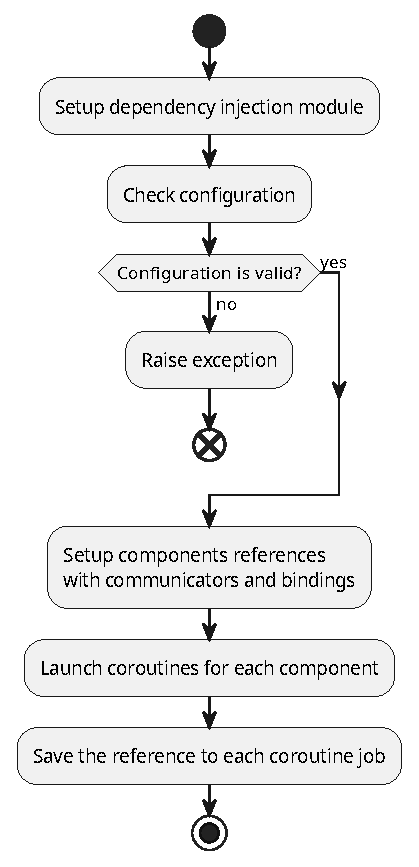
\includegraphics[width=0.4\textwidth]{figures/platform-setup-sequence.pdf}
	\caption{Activity diagram showing the platform creation process.}
	\label{fig:platform-configuration}
\end{figure}

The creation of component references for the behavior component, requires further analysis: in fact, the behaviour holds a reference for each
component, namely the \emph{state, actuators, sensors,} and \emph{communication}.
In this regard, not all four components might be defined, so the behavior will have to create a dummy component reference for the missing components.
This is managed automatically when creating component references by looking at the configuration, and if a component is neither local nor remote,
then the dummy implementation is used.

% - New section ---------------------------------------------------------------

\section{RabbitMQ module}
\label{sec:rabbitmq-module-impl}

The RabbitMQ module, at the time of writing, is the only module that provides an implementation of the \texttt{Communicator} interface.
In particular, this module enables the communication between components via \textbf{RabbitMQ}, a message broker that implements the AMQP protocol.

\subsubsection{RabbitMQ overview}

RabbiMQ is an open source \textbf{message broker} written in Erlang that implements the \textbf{AMQP} protocol~\cite{4012603}.
RabbitMQ is lightweight and easy to deploy on-premises and in the cloud. It supports multiple messaging protocols. RabbitMQ can be deployed in
distributed and federated configurations to meet high-scale, high-availability requirements~\footnote{\url{https://www.rabbitmq.com/\#features}}.

RabbitMQ is based on the notion of \textbf{broker}, which receives messages from publishers (applications that publish them, also known as producers)
and route them to consumers (applications that process them). The publishers, consumers and the broker can all reside on different machines,
reasons why RabbitMQ could be a good choice for a distributed system, in particular in the context of the pulverization.

The AMQP protocol has the following view of the world: messages are published to exchanges, which are often compared to post offices or mailboxes.
\emph{Exchanges} then distribute message copies to queues using rules called bindings. Then the broker either delivers messages to consumers
subscribed to queues or consumers fetch/pull messages from queues on demand.

Networks are unreliable and applications may fail to process messages therefore the AMQP model has a notion of message acknowledgments: when a
message is delivered to a consumer the consumer notifies the broker, either automatically or as soon as the application developer chooses to do so.
When message acknowledgements are in use, a broker will only completely remove a message from a queue when it receives a notification for that
message (or group of messages).

Exchanges are entities that receive messages from producers and route them to zero or more queues. The routing algorithm depends on the exchange
type and rules called bindings. The AMQP protocol defines four exchange types that are reported in~\Cref{tab:exchange-types}.

\begin{table}[ht]
	\centering
	\begin{tabular}{l l}
		\toprule
		\textbf{Exchange type} & \textbf{Default names}                                    \\
		\midrule
		Direct exchange        & (Empty string) and \texttt{amq.direct}                    \\
		Fanout exchange        & \texttt{amq.fanout}                                       \\
		Topic exchange         & \texttt{amq.topic}                                        \\
		Headers exchange       & \texttt{amq.match} (and \texttt{amq.headers} in RabbitMQ) \\
		\bottomrule
	\end{tabular}
	\caption{Exchange types.}
	\label{tab:exchange-types}
\end{table}

The \emph{default exchange} is a direct exchange with no name (empty string) pre-declared by the broker. It has one special property that makes it
very useful for simple applications: every queue that is created is automatically bound to it with a routing key which is the same as the queue name.

\begin{figure}[h!]
	\centering
	\begin{subfigure}{.45\textwidth}
		\centering
		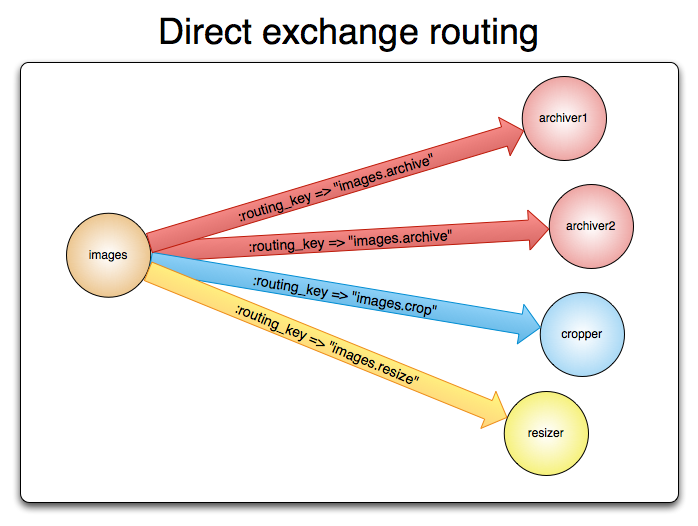
\includegraphics[width=0.84\linewidth]{figures/exchange-direct.png}
		\caption{Direct exchange example.}
		\label{fig:direc-exchange}
	\end{subfigure}
	\begin{subfigure}{.45\textwidth}
		\centering
		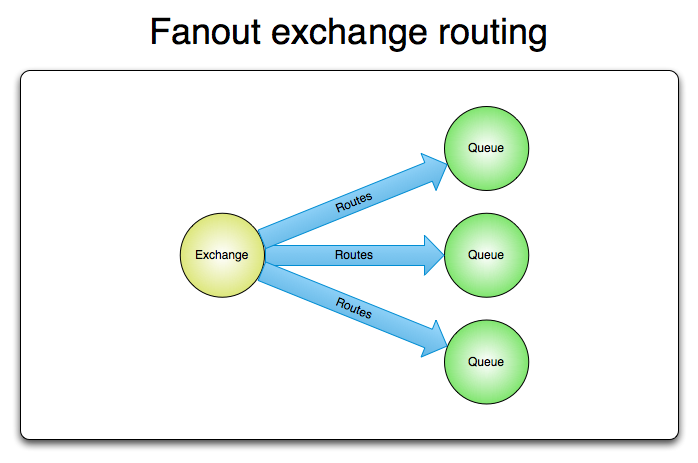
\includegraphics[width=\linewidth]{figures/exchange-fanout.png}
		\caption{Fanout exchange example.}
		\label{fig:fanout-exchange}
	\end{subfigure}
	\caption{Representation of the two main exchanges defined in the AMQP protocol. Pictures taken from~\cite{rabbitmq-amqp-concepts}.}
	\label{fig:amqp-exhange-type}
\end{figure}

A direct exchange delivers messages to queues based on the message routing key.
A direct exchange is ideal for the unicast routing of messages (although they can be used for multicast routing as well).
Below is reported how a direct exchange works:

\begin{itemize}
	\item A queue binds to the exchange with a routing key $K$
	\item When a new message with routing key $R$ arrives at the direct exchange, the exchange routes it to the queue if $K = R$
\end{itemize}

A direct exchange can be represented graphically as in~\Cref{fig:direc-exchange}.

A fanout exchange routes messages to all of the queues that are bound to it and the routing key is ignored. If $N$ queues are bound to a fanout
exchange, when a new message is published to that exchange a copy of the message is delivered to all $N$ queues. Fanout exchanges are ideal for the
broadcast routing of messages. A fanout exchange can be represented graphically as in~\Cref{fig:fanout-exchange}.

Topic exchanges route messages to one or many queues based on matching between a message routing key and the pattern that was used to bind a queue to
an exchange. The topic exchange type is often used to implement various publish/subscribe pattern variations. Topic exchanges are commonly used for
the multicast routing of messages. Whenever a problem involves multiple consumers/applications that selectively choose which type of messages they
want to receive, the use of topic exchanges should be considered.

\subsubsection{Rabbimq communicator}

\hyphenation{default-RabbitMQ-Remote-Place}

When implementing a new \texttt{Communicator}, two main steps are required: the first one is the implementation of the \texttt{Communicator} interface
and the second one is the implementation of the \texttt{RemotePlaceProvider}.
The \texttt{Communicator} interface is implemented by the \texttt{RabbitMQCommunicator} class, while the default implementation of the
\texttt{RemotePlaceProvider} interface is provided by the \texttt{default\-RabbitMQ\-Remote\-Place} method.

The remote place provider provides the implementation of the concepts ``who'' and ``where'' (defined by the \texttt{RemotePlace} class) in the
following way: the \texttt{who} is the \emph{device id}, while the \texttt{where} is the \emph{name of the component}.
This representation will be used by the \texttt{RabbitmqCommunicator} to create the queues that will be used to communicate between the components.

The \texttt{RabbitmqCommunicator} should rely on a library that implements the AMQP protocol to communicate with the RabbitMQ broker, but since
there isn't a Kotlin multiplatform library that implements the AMQP protocol, the class is marked as \texttt{expect} so that the specific target
platform can provide the implementation. At the time of writing, only the JVM target platform is implemented using the \texttt{reactor-rabbitmq}
library. The choice of this library is because it is based on project \emph{Reactor}~\footnote{\url{https://projectreactor.io/}} and can be
seamlessly used in combination with the Kotlin coroutines using the
\texttt{kotlinx-coroutine-reactor}~\footnote{\url{https://kotlinlang.org/api/kotlinx.coroutines/kotlinx-coroutines-reactor/}} library.

The class constructor accepts all the RabbitMQ-specific parameters like: \emph{host}, \emph{port}, \emph{username}, \emph{password}, and
\emph{virtual host}.
Noticeable is the \texttt{setup} method that is used to set up the connection with the RabbitMQ broker, declare the exchange and the queues, and
finally bind the queues to the exchange. In this method, the \texttt{binding} and the \texttt{remote place} are used to create the queues that will
be used to communicate between the components.

Below will be described how the queues are created and how they are used to communicate between the components.
The \texttt{RabbitmqCommunicator} class defines two queues: a \emph{sendQueue} and a \emph{receiveQueue}, the first one is used to send messages to
the remote component, while the second one is used to receive messages from the remote component.
In this communicator, the send queue name format follows the pattern \texttt{<local component name>/<remote component name>/<remote component id},
while the receive queue name format follows the pattern \texttt{<remote component name>/<local component name>/<remote component id>}.
The \emph{local component name} is retrieved from the \texttt{binding} parameter, while the \emph{remote component name} and the
\emph{remote component id} are retrieved from the \texttt{remote place} parameter.
For example, if the communicator should manage the communication between the \emph{Behaviour} and the \emph{State} (remote) component for a device
with ID ``1'', the send queue name will be \texttt{Behaviour/State/1}, while the receive queue name will be \texttt{State/Behaviour/1}.
Vice versa, the counterpart communicator that manages the communication between the \emph{State} and the \emph{Behaviour} (remote) component
defines the send queue name as \texttt{State/Behaviour/1} and the receive queue name as \texttt{Behaviour/State/1}.
As can be seen, the send queue name for the first communicator is the same as the receive queue name for the counterpart communicator, and vice versa.
This means that the message sent by the first communicator will be received by the counterpart communicator.
The~\Cref{fig:rabbitmq-queues} depicts the interaction pattern described above using two communicators.

\begin{figure}[ht]
	\centering
	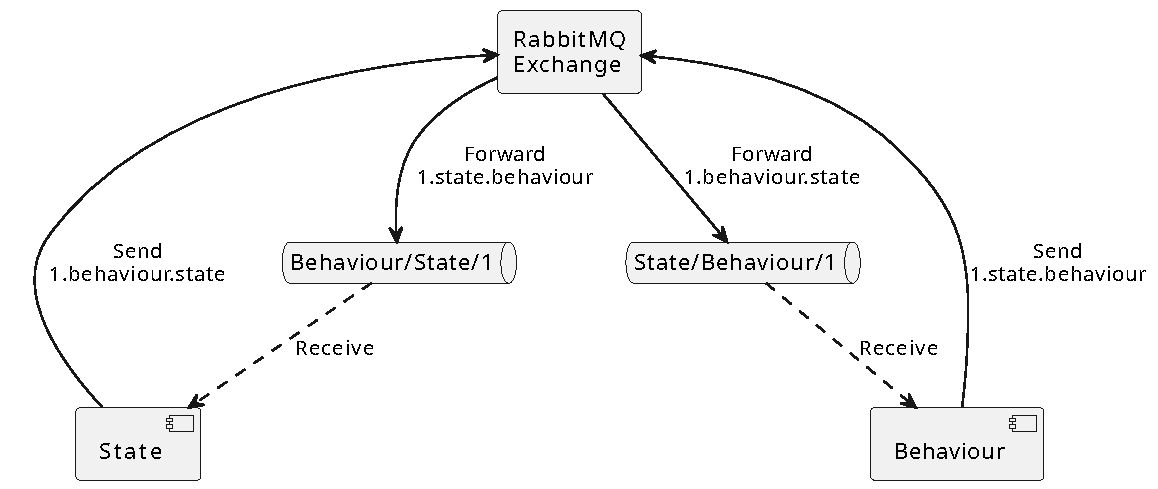
\includegraphics[width=\textwidth]{figures/rabbitmq-queue.pdf}
	\caption{RabbitMQ queues}
	\label{fig:rabbitmq-queues}
\end{figure}

The \texttt{fireMessage} and \texttt{receiveMessage} methods implementation are straightforward: the \texttt{fireMessage} method sends the message
to the remote component via the send queue using the \texttt{Sender} object, while the \texttt{receiveMessage} method receives the message from the
remote component via the receive queue using the \texttt{Receiver} object.

% - New section ---------------------------------------------------------------

\section{Configuration DSL}
\label{sec:configuration-dsl-impl}

\hyphenation{Device-Relations-Configuration}
\hyphenation{Logical-Device-Configuration}

The configuration DSL is used to define the structure of each logical device in terms of defining components and where they are deployed.
Before proceeding to discuss the details of the DSL, it is important to define which information the configuration should have.

The recurring terms and concepts in the pulverization are \emph{logical device}, \emph{deployment unit} and \emph{place} where the components are
deployed. The first concept is modeled by the \texttt{LogicalDeviceConfiguration} class which defines the name of the device, the set of components
type belonging to the logical device, and a set of deployment units.
The \emph{deployment unit} is modeled by the \texttt{DeploymentUnit} class which defines the set of components type that should be deployed and the
\texttt{Tier} which represents the place where the components should be deployed. The \emph{tier} is modeled via a sealed interface which has
three possible values: \texttt{Cloud}, \texttt{Edge} and \texttt{Device}.

The configuration captures also the concept of ``relationship'' between logical devices. In particular, the configuration DSL defines
the \texttt{Device\-Relations\-Configuration} and the \texttt{DeviceLink} classes which are used to hold information about the link between the logical devices.

Finally, the \texttt{PulverizationConfiguration} class has a set of \texttt{Logical\-Device\-Configuration} and a
\texttt{DeviceRelationsConfiguration}; this class represents the root of the configuration and is used to configure the pulverization platform.
The~\Cref{fig:configuration-dsl-classes} depicts the relationship between the classes that define the configuration that can be created via the
configuration DSL.

\begin{figure}[h]
	\centering
	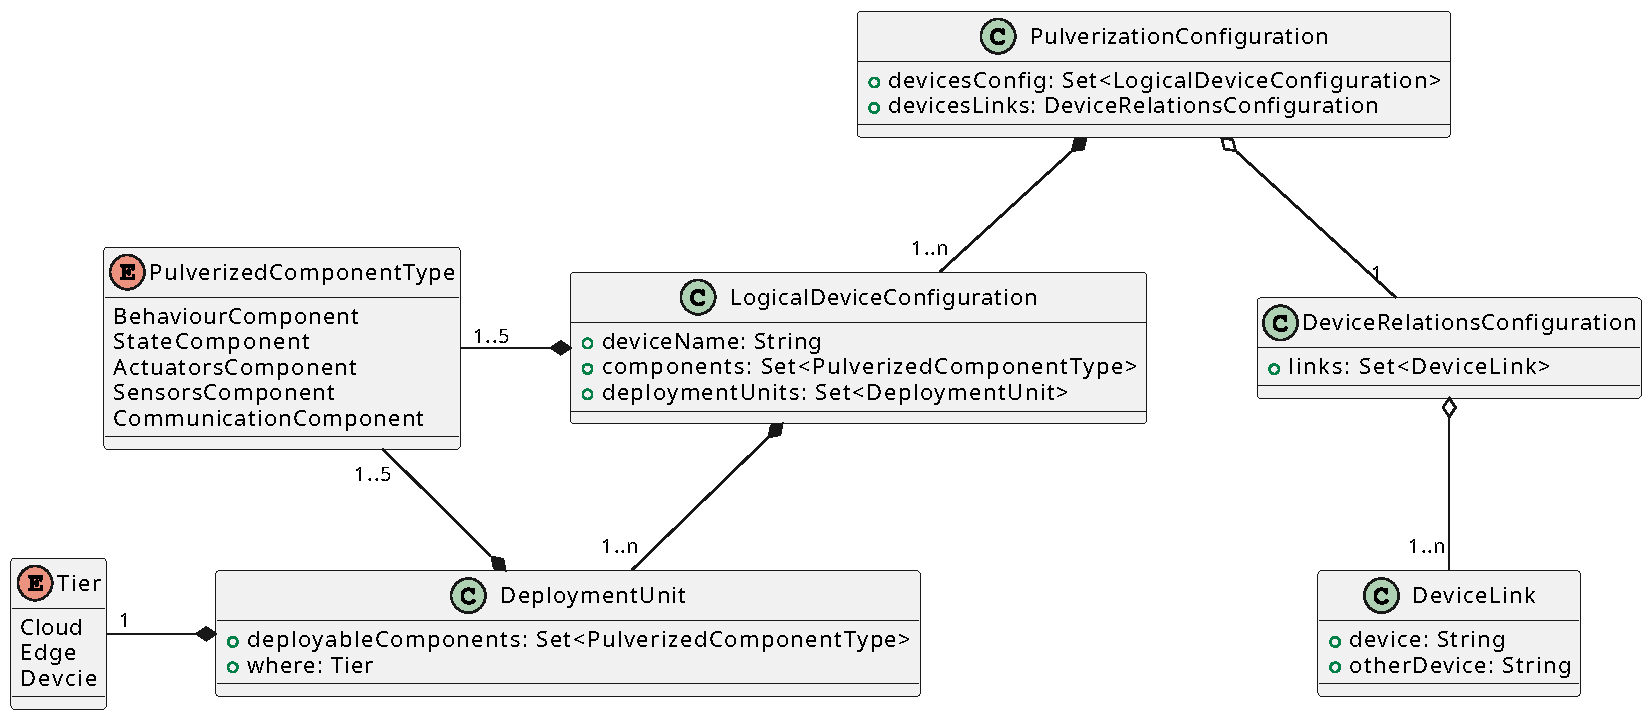
\includegraphics[width=\textwidth]{figures/config-dsl-class.pdf}
	\caption{Configuration DSL class diagram.}
	\label{fig:configuration-dsl-classes}
\end{figure}

The configuration is enriched with some extension methods that allow getting the logical device configuration from a given device name and
from a logical device configuration, can be retrieved the deployment unit from the given components.

An example of configuration is shown on the~\Cref{lst:configuration-dsl-impl}. The configuration defines three logical devices where the
\emph{device-1} can communicate with the \emph{device-2} and the \emph{device-3}. At the time of writing, the information about the links
between the logical devices is not used by the framework, but in a future version, this information can be used, for example, by the communication
components to establish the right communication within the network.

\lstinputlisting[
	float=h,
	language=Kotlin,
	caption={Configuration DSL},
	label={lst:configuration-dsl-impl}
]{listings/configuration-dsl.kt}

% - New section ---------------------------------------------------------------

\section{Platform DSL}
\label{sec:platform-dsl-impl}

The platform DSL represents one fundamental building block of the entire framework: with this DSL the user can configure the platform in a simple
declarative way, without the need to manage specific aspects like how the components should be instantiated or how the communication between them
should occur. The DSL is implemented in the \emph{dsl} package of the \emph{platform} module and should provide the following features:

\begin{itemize}
	\item The ability to register the user-defined components with their corresponding logic
	\item The ability to specify which communicator should be used to communicate between the components
	\item The ability to specify a custom context that should be used.
	\item Produce a platform instance that can be used to start the pulverized system.
\end{itemize}

All of those four features are implemented in the DSL using the syntax and the structure defined in the~\Cref{lst:platform-dsl} which provides
an example of the use of the DSL to configure the platform.

\lstinputlisting[
	float=h,
	language=Kotlin,
	caption={Example of the use of the DSL to configure the platform.},
	label={lst:platform-dsl}
]{listings/PlatformDSL.kt}

First of all, the DSL takes as arguments the configuration of the device that should be executed; the configuration is used to know which components
the logical device has and how they are distributed across the infrastructure. With that information, the platform can determine which components
are local (in the same deployment unit) and which are remote, instantiating the right components and communicators.

Then, the DSL provides a way to register the user-defined components with their corresponding logic. If the given components do not match the
configuration, an exception is raised.

Finally, the type of communicator and the remote place provider can be specified respectively via the \texttt{withPlatform} and
\texttt{withRemotePlace} methods. The context can be overridden via the \texttt{withContext} method.

The development of this DSL has involved the resolution of several issues, in particular, the management of serialization aspects and a limitation of
the Kotlin type inference. Below are described those issues and the solutions adopted to overcome them.

\subsubsection{Serialization}

Serialization represents an important aspect of the working of the framework but at the same time, you don't want to force the user to manage
serialization aspects. Is the responsibility of the framework to retrieve the serializer from the user-defined components and to use it in
conjunction with other framework elements like the communicators. Thus, the low complexity of using and configuring the framework is guaranteed.

The first issue is how to retrieve the serializer from the user-defined components without forcing the user to provide it. The solution adopted
defines the DSL entry point as an inline function that accepts a reified type parameter, in this way, the serializer can be retrieved via the
\texttt{serializer} method. In particular, the function defines five type parameters: \texttt{S, C, SS, AS,} and \texttt{R} which respectively
represents the type of the state, the type of communication, the type of the sensors, the type of the actuators, and the type of behaviour result.

The problem occurs when a logical device does not define all of the five components but only a subset of them.
For example, if a logical device is made of the \emph{behaviour, communication, sensors,} and \emph{actuators} components when using the DSL, a type
for the \emph{state} should be provided. A first, elegant approach would be to default all the unspecified types to the \texttt{Nothing} bottom type;
however, this approach is not feasible, since the \texttt{Nothing} type is not serializable and thus, it cannot be inlined as a type.
The solution adopted is to use \texttt{Any} as the default type for the unspecified components. This solution enables the inlining of the type,
so the function can be used (as inline) but the drawback is that there is no serializer for the \texttt{Any} type.
Since the absence of the type means that the component is not used, the serializer for the \texttt{Any} type is a dummy serializer that does
nothing but makes the function sound. In this way, a check can be made to verify if the given type is \texttt{Any} (and rely on the dummy serializer)
or if it is a specified type retrieving the serializer from it.

The~\Cref{lst:any-serializer} shows the implementation of the dummy serializer for the \texttt{Any} type and how the serializer is retrieved from the
user-defined types.

\lstinputlisting[
	float=h,
	language=Kotlin,
	caption={Dummy serializer for the Any type.},
	label={lst:any-serializer}
]{listings/AnySerializer.kt}

\subsubsection{Type inference problem}

The second issue is related to the type inference of Kotlin that does not infer a default type for an unspecified generic type.
As said in the previous sections, the simplicity of the use of the DSL is one of the main goals of the framework. In particular, when the user
configures the platform using the DSL, the user does not need to specify the type of components, since the framework can infer them from the
configuration. However, the Kotlin type inference does not work for the generic types that are not specified raising a compilation error, forcing
to specify all the types required by the entry point function of the DSL. The~\Cref{lst:platform-dsl-verbose} shows an example of the use of the
DSL when all the types are specified. The proposed example although valid and works, is not very elegant because forces the user to remember
the positional order of the types and specify all of them.

To minimize the amount of boilerplate code and maintain the simplicity of the DSL, the proposed solution utilizes extension methods to
facilitate type inference for all five types included in the user-defined configuration base.
With the use of the extension methods, the Kotlin type inference algorithm can infer the right types without specifying them explicitly.
This is a sort of workaround to deal with the limitation of the Kotlin type inference algorithm that does not infer a default type for an
unspecified generic type.

\lstinputlisting[
	float=h,
	language=Kotlin,
	caption={Example of the verbosity of the DSL when all the types are specified.},
	label={lst:platform-dsl-verbose}
]{listings/dsl-verbose.kt}

The~\Cref{lst:platform-dsl-inference} shows the implementation of the extension methods that help the type inference to infer the
right types without specifying them explicitly.

\lstinputlisting[
	float=h,
	language=Kotlin,
	caption={Extension methods to help the Kotlin type inference algorithm.},
	label={lst:platform-dsl-inference}
]{listings/dsl-type-inference.kt}
